\documentclass{article}
\usepackage{geometry}
\geometry{a4paper, top=3cm, bottom=3cm, left=2cm, right=2cm}
\usepackage[utf8]{inputenc}
\usepackage[english]{babel}
\usepackage{hyperref}
\makeindex

\title{Image Processing and Computer Graphics}
\author{Riccardo Salvalaggio}
\date{19th of April, 2021}

\usepackage{wrapfig}
\usepackage{amssymb}
\usepackage{amsmath}
\usepackage{txfonts}
\usepackage{mathdots}
\usepackage{graphicx}
\newtheorem{theorem}{Lambert's Cosine Law}

\begin{document}

\maketitle
\newpage
\tableofcontents
\newpage

\part{Computer Graphics}
\newpage
\section{Introduction Computer Graphics}
Modeling: generate, represent geometry.\\
Rendering: light transposing, delete objects etc.\\
Simulation: animation, dynamic representation.\\

\textbf{Light:} energy or photons generated by a source, transported along lines, interacting at surfaces (reflection).\\
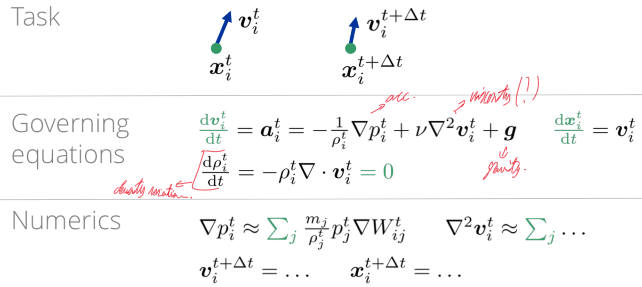
\includegraphics{image1.png}
Pressure is computed by solving a pressure Poisson equation.

\subsection{Rendering aspects}
- Ray Tracing: \\
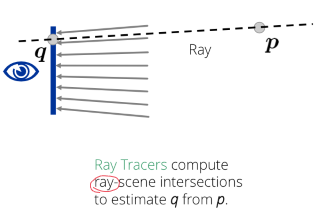
\includegraphics{image4.png}\\
- Rasterization: \\
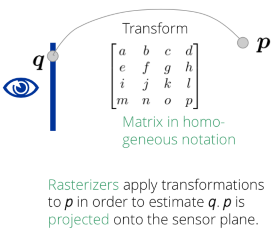
\includegraphics{image5.png}


\subsection{Light}
Photons are characterized by a wavelength within the visible spectrum => color.\\

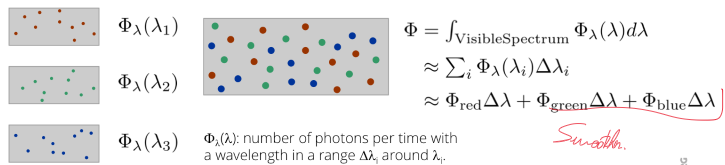
\includegraphics{image2.png}
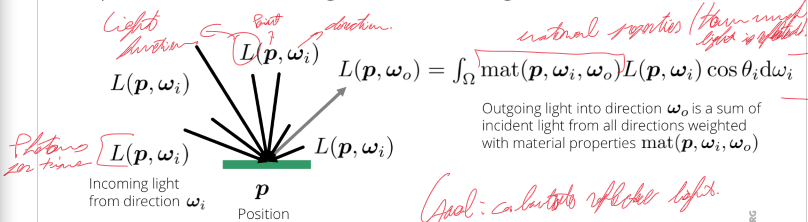
\includegraphics{image3.png}

Rendering -> lookup light transported along rays casted into the scene.
\newpage
\section{Ray Casting}
Rendering problem: visibility/hidden surface problem, object projection onto sensor plane. (Rat-object intersections with ray casting/tracing).\\
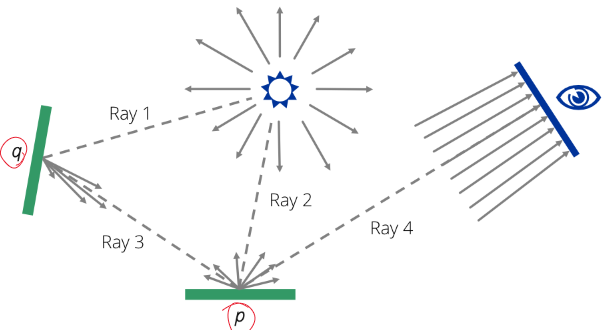
\includegraphics{image6.png}
\textbf{Goal:} to compute ray 4 (incoming light at the sensor considering every riflection).\\
Increasing the number of rays we are considering, we obtain an higher precision (great computationally effort).\\
\textbf{Primary rays: } start/end at sensors\\
\textbf{Secondary rays: } don't start/end at sensors\\
\textbf{Shadow rays: } start/end at sources\\
Primary solve visibility problem, secondary are useful in order to compute light transport.\\
\textbf{Ray casting: }computation of position p (what is visible).\\
\textbf{Ray tracing: }computaiton of light transportd (which colors).\\
Rendering equations to compue incoming light.
\textbf{Concept: }a ray is a half-line specified by an origin o and a direction d => r(t) = o+td with t>=0. We have to compute nearest intersection with all objects.
\subsection{Implicit surfaces}
If p = x,y,z is a surface point => f(x,y,z) = 0.\\
Intersection: f(x,y,z) = f(r(t)) = f(o+td) = 0. All point on a normal surface with offset r satisfy that intersection => n*(p-r) = 0. If d is not orthogonal to n, the intersection can be computed: n*(o+td-r)=0, t=[(r-o)*n]/[n*d].\\
n is given by gradient ( function that compute the variation for unit) of the implicit function (n is the direction with the greater value of gradient).\\
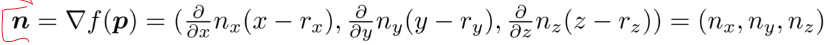
\includegraphics{image7.png}
For quadrics we use the same knowledge expanded to three dimensions (quadratic equations).\\
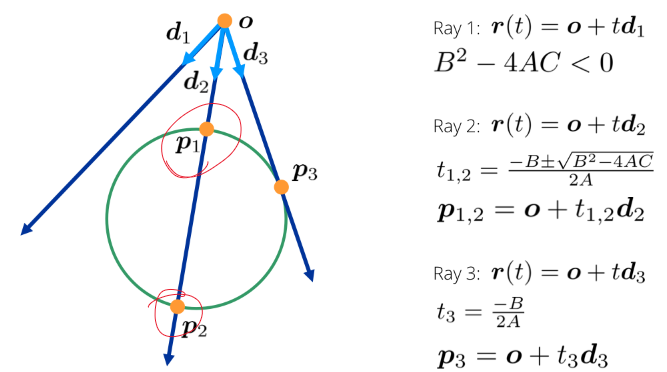
\includegraphics{image8.png}
\subsection{Parametric surfaces}
Represented by functions with 2D parameters: x = f(u,v), y = g(u,v), z = h(u,v)\\
Intersetion can be computer from a non-linear system.\\
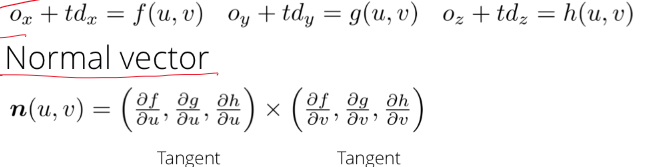
\includegraphics{image9.png}
Parametric representations are used to render partial objects.
\subsection{Combined objects}
\textbf{Compound objects: }union of forms.\\
\textbf{Constructive Solid Geomtry CSG: }combine simple objects to complex geometry using boolean operators.\\
Estimate and analyze all intersections considering intervals inside objects, works for closed surfaces.
\subsection{Triangles}
Popular appoximate surface representation
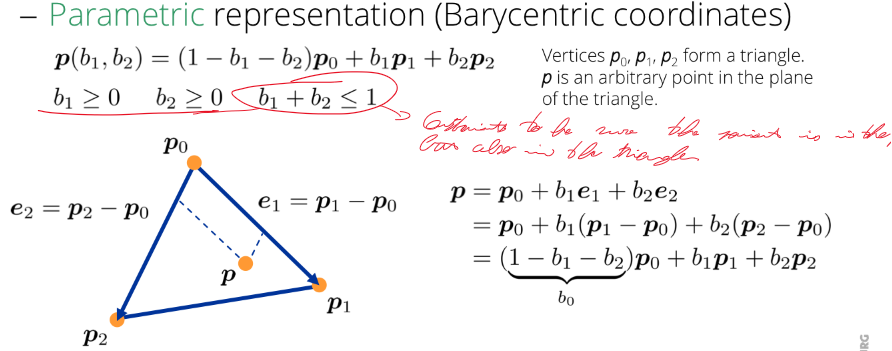
\includegraphics{image10.png}
Intersection: o+td = (1-b1-b2)p0 + b1p1 + b2p2. \\
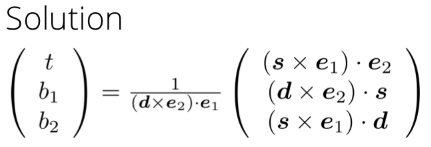
\includegraphics{image11.png}
\subsection{Axis-aligned boxes}
\subsubsection{Axis-Aligned Bounding Box (AABB)}
Simple geometry outside complex geometry, if a ray doesn't intersecate to the simple, surely doesn't intersect the complex. Boxes are represented by slabs. Intersections of rays are analyzed in order to check for ray-object intersection.
Implementations is again done using normal intersection equation.
Overlapping ray intervals indicate intrsections.\\
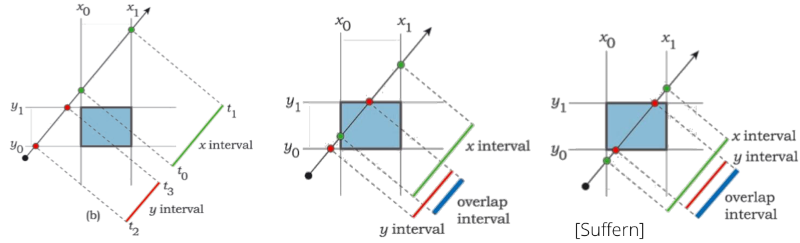
\includegraphics{image12.png}
\subsubsection{Bounding Volume Hierarchies (BVH)}
AABBs combined in a hierarchy way. put smaller boxes recursively. Efficient pruning but memory and pre-processing overhead.
\subsection{Iso-surfaces in grids}
In order to compute intersections on fluid surfaces. Computation is based on density comparison.\\\\
Ray casting is very versatile concept to compute what is visible at a sensor but so expensive for complex geometries.

\section{Shading}
The way to compute color and intensity of what is visible by the sensor. Light is emitted by light sources but is scattered and or absorbed by surface (if dark aborbed, if bright reflected)and media.\\
Radiance: photons per time * area * solid angle (describe how much light is transported).
\textbf{Coloured light }is represented by a 3D vector L: (Lred, Lgreen, Lblue).
\textbf{Coloured objects }are characterized by reflectance coefficient $\rho$ = ($\rho$red, $\rho$green, $\rho$blue). Colours that are in the vector are reflected, otherwise absorbed.\\
We'll use Local Illumination Models that approximately solve the rendering equation.\\
\subsection{Phong Illumination Model}
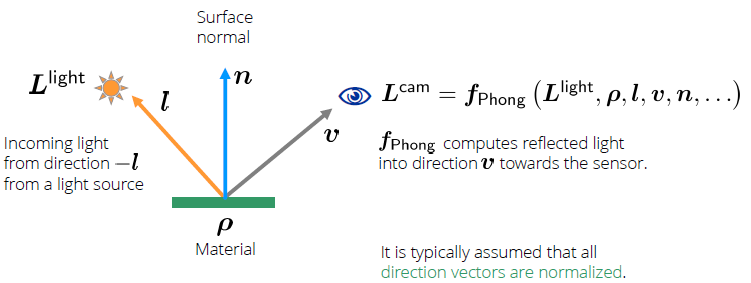
\includegraphics{image13.png}\\
Lsurf is the surface illumination caused by Llight. Lrefl will depend on the object color $\rho$. Lcam is a portion of Lrefl transported to the sensor (will depend on the material).

\begin{theorem}
Illumination strenght at a surface is proportional to the cosine of the angle between l and n.
\end{theorem}
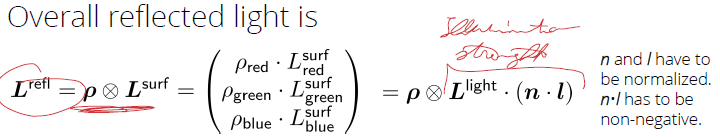
\includegraphics[scale=0.6]{image14.png}\\
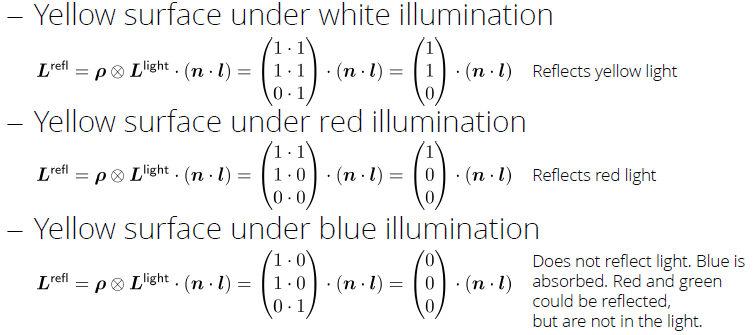
\includegraphics[scale=0.6]{image15.png}\\
Depending on the material, the reflection will be either Diffuse (if Matte) or Specular (if Shiny).\\\\
\subsubsection{Diffuse Reflection}
Matte surfaces reflect light equally into all directions.\\
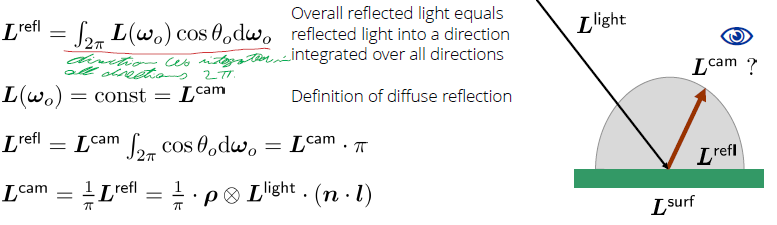
\includegraphics[scale=0.6]{image16.png}\\
\subsubsection{Specular Reflection}
Shiny surfaces reflect light into a small set of dominant directions.\\
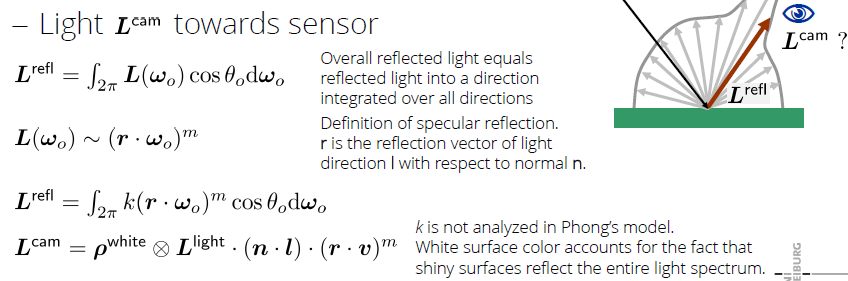
\includegraphics[scale=0.6]{image17.png}\\
Exponent m governs the size of the highlight area. M does not influence the maximal intensity. r can be computed as: r = 2*(l*n)*n-l.\\
According to the Blinn-Phong (Lrefl from a shiny surface) illumination model r = (l+v)/norma(l+v).\\
\subsubsection{Reflection from Ambient Illumination}
Indirect illumination from other surfaces. Reflecte light is: p$\_xor$Lindirect.\\
Lcam = 1/$\_pi$*p$\_xor$Lindirect.
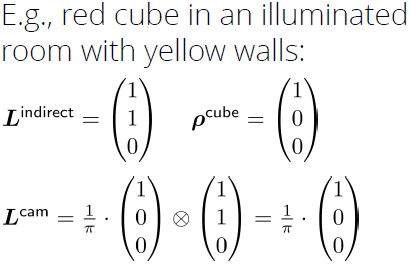
\includegraphics[scale=0.6]{image18.png}
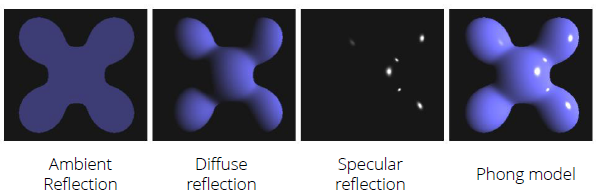
\includegraphics[scale=0.6]{image19.png}\\
\begin{figure}
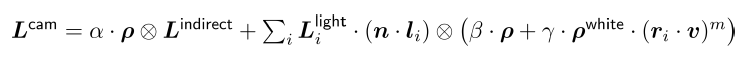
\includegraphics[scale=0.6]{image20.png}
\caption{Total model (coefficients are user-defined)}
\end{figure}
In conclusion Phong is an efficient local computing model and its implementation can be parallelized.Drawbacks: resulting images tend to look less realistic because realistic scenes have more complex illuminations, complex material and non-physical phong parameters cause issues.\\

\subsection{Extensions}
Distances must be considered:\\
1. Between object surface and light source.\\
- Inverse Square Law: Illumination of a surface decreases quadratically with the distance from a light source =\textgreater Lsurf = $(1/r^2)*Llight*(n*l)$.\\
2. Between object surface and viewer.\\
- Fog: It is approximated by a combination of Lcam and Cfog. Lcam,fog = f(d)*Lcam+(1-f(d))*Cfog. f(d) describes the visibility.
\subsection{Shading Models} 
Illumination models can be evaluated per vertex or per fragment.\\
Faces/primitives are characterized by vertices.\\
Projected area of a face onto the sensor is subdivided into fragments.\\
Shading models specify whether the illumination model is evaluated per vertex or per fragment:\\
- If evaluated per vertex, the shading model specifies whether the resulting vertex colors are interpolated across a primitive or not.\\
- If evaluated per fragment, surface normals are interpolated across a primitive.\\
\subsubsection{Well-knows Models}
- Flat shading: evaluation per vertex, fragments are colored with the color of one specific vertex.\\
- Gouraud shading: evaluation per vertex, fragments are interpolated from vertex colors.\\ 
- Phong shading: evaluation per fragment, normals have to be interpolated from vertices to fragments.

\section{Homogeneous Notation}
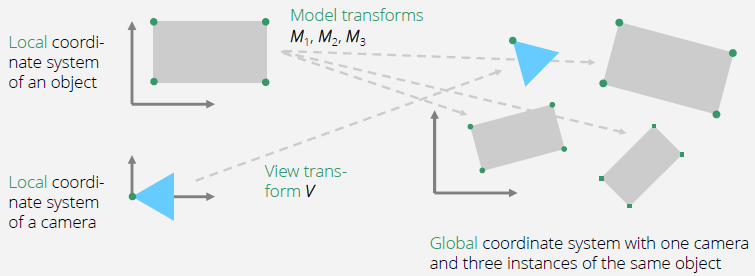
\includegraphics[scale=0.6]{image21.png}\\\\
To transform from view space positions to positions on the camera plane:\\
- Projection transform\\
- Viewport transform\\
Affine trasformatiokns: angles and lengths are not preserved, collinearity, proportions, parallelism are.\\
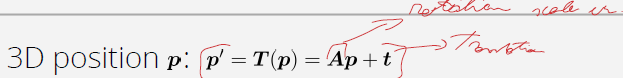
\includegraphics[scale=0.6]{image22.png}\\\\
3x3 matrix A represents linear transformations, 3D vector t represents translation. Using the homogeneous notation, all affine transformations are represented with one matrix vector multiplication.\\
Using the homogeneous notation, transformations of vectors and positions are handled in a unified way.\\
- From Cartesian to Homogeneous:\\
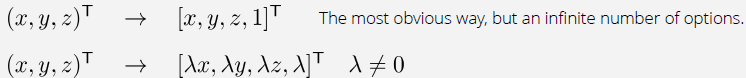
\includegraphics[scale=0.6]{image23.png}\\\\
- From Homogeneous to Cartesian:\\
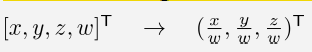
\includegraphics[scale=0.6]{image24.png}\\\\
\begin{figure}
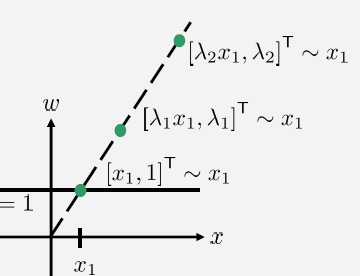
\includegraphics[scale=0.6]{image25.png}
\caption{1D Illustration}
\end{figure}
- General form:\\
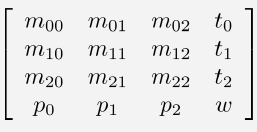
\includegraphics[scale=0.6]{image26.png}\\
m is rotation,scale,shear; t is translation; p for projection; w is the homogeneous component.\\

\subsection{Transformations}
\subsubsection{Translation}
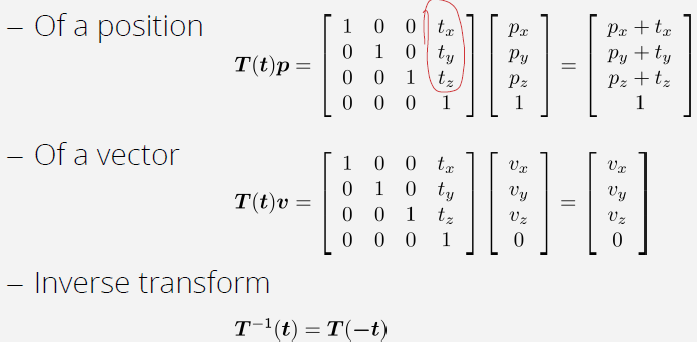
\includegraphics[scale=0.6]{image27.png}\\
\subsubsection{Rotation}
Positive (anticlockwise)\\
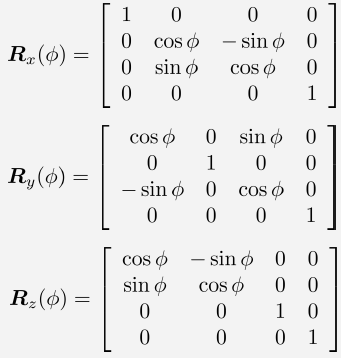
\includegraphics[scale=0.6]{image28.png}\\
\subsubsection{Mirroring}
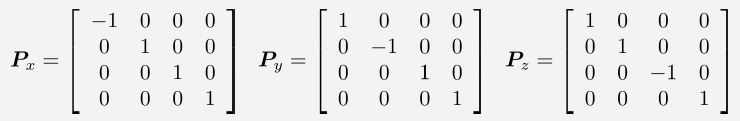
\includegraphics[scale=0.6]{image29.png}\\\\
Rotation and reflection matrices are orthogonal: $RR^T=R^TR=I, R^-1=R^T$
\subsubsection{Scale}
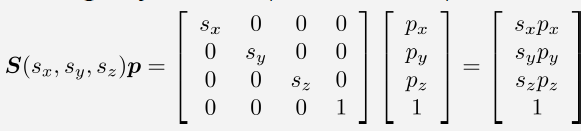
\includegraphics[scale=0.6]{image30.png}\\\\
\subsubsection{Shear}
Offset of one component wrt another component.\\
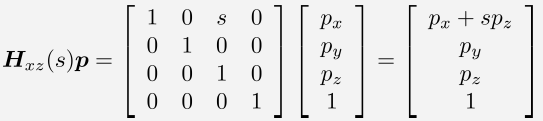
\includegraphics[scale=0.6]{image31.png}\\\\
\textbf{Example:}\\\\
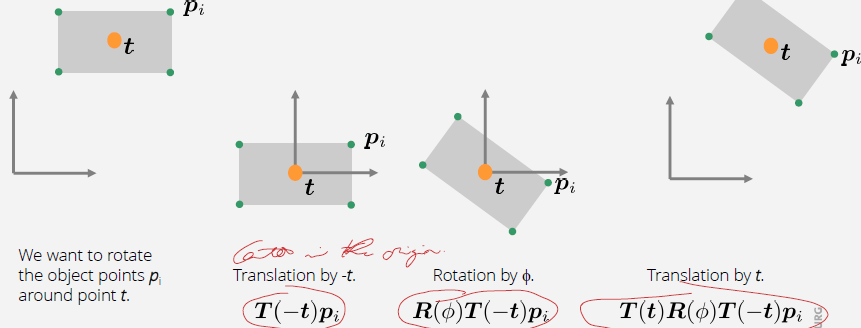
\includegraphics[scale=0.6]{image32.png}\\\\
\subsubsection{Planes and normals}
Planes can be represented by a surface normal n and a point r. All points p with n*(p-r)=0 form a plane.\\
\subsubsection{Basis Transform}
- Translation\\
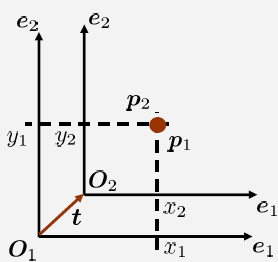
\includegraphics[scale=0.6]{image33.png}\\\\
- Rotation\\
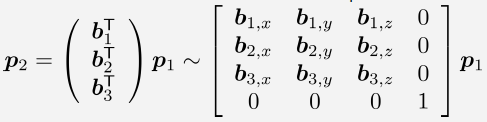
\includegraphics[scale=0.6]{image34.png}\\\\
The view transform can be seen as a basis transform. Placing and orienting the camera is a transformation v.The basis transform is realized by applying $v^-1$ to all objects.\\
Usage of the homogeneous notation is motivated by a unified processing of affine transformations, perspective projections, points, and vectors.All transformations of points and vectors are represented by a matrix vector multiplication.\\

\section{Projection}
Last matrix M row is dedicated to projections and can be used to realize divisions by a linear combination.\\
\begin{figure}
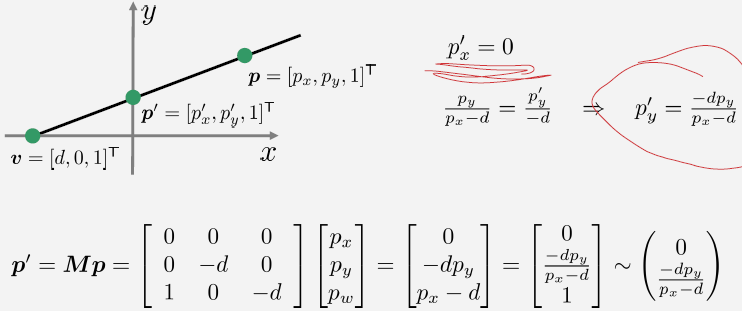
\includegraphics[scale=0.6]{image35.png}
\caption{To compute intersection with the x-axis}
\end{figure}
\subsection{2D projections}
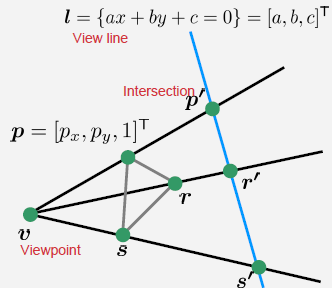
\includegraphics[scale=0.6]{image36.png}\\\\
If the homogeneous component of v is not equal to zero, we have a perspective projection; if v is at infinity, we have a parallel projection.\\
Location of viewpoint and orientation of the viewline determine the type of projection:\\
- Parallel (viewpoint at infinity, parallel projectors).\\
	- Orthographic (viewline orthogonal to the projectors).\\
	- Oblique (viewline not orthogonal to the projectors).\\
- Perspective (non parallel projectors):\\
	- One point (viewline intersects one principal axis).\\
	- Two point (viewline intersects two principal axes, two vanishing points).\\\\
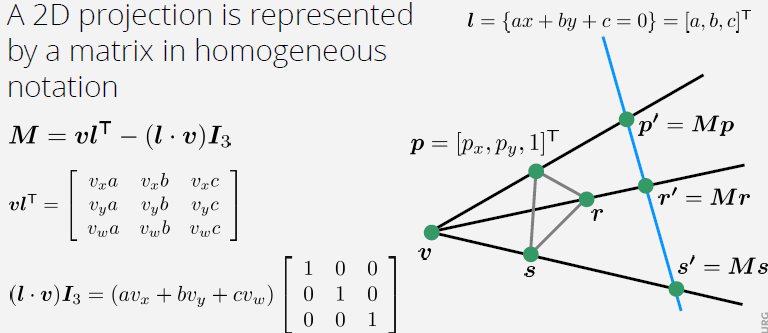
\includegraphics[scale=0.6]{image37.png}\\\\
See other examples on slides.\\\\

\subsection{3D projections}
Same thing expanded to 3D.\\\\
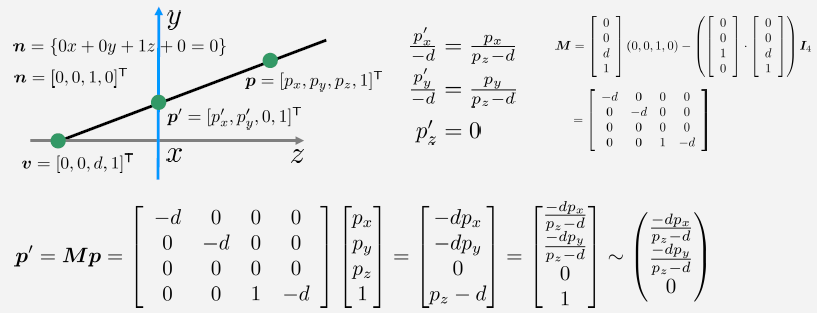
\includegraphics[scale=0.6]{image38.png}\\\\
\subsection{Projection Transform}
\subsubsection{Modelview Transformation}
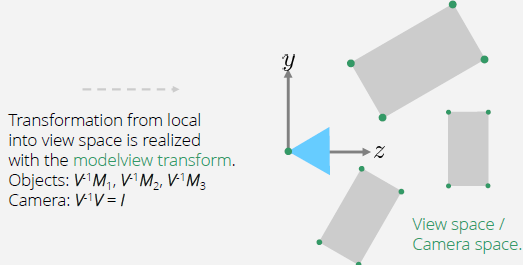
\includegraphics[scale=0.6]{image39.png}\\\\
\subsubsection{Projection Transformation}
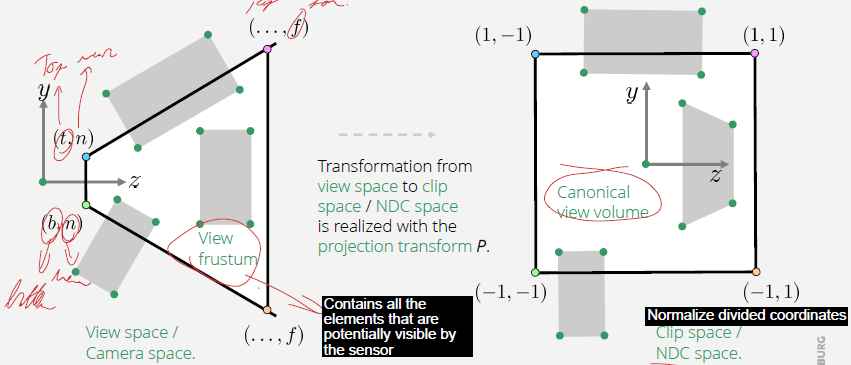
\includegraphics[scale=0.6]{image40.png}\\\\
Why to transform to Clip/NDC? It allows simplified and unified implementations:\\
Culling (exclude non-visible elements), Clipping (exclude non-visible parts of visible elements), Visibility (useful for ray tracing).\\
\subsubsection{Perspective Projection Transformation}
Maps a view volume/pyramidal frustum (l,r,t,b) to a canonical view volume (-1,1). It is applied to vertices. Maps coordinates to (-1,1) maintaining coherence.\\

- Derivation \\\\
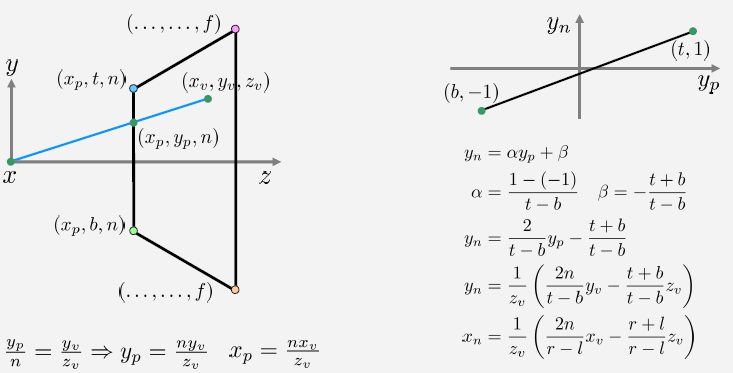
\includegraphics[scale=0.6]{image41.png}\\\\
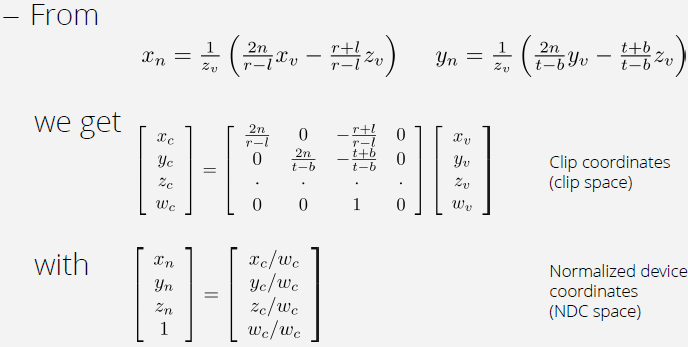
\includegraphics[scale=0.6]{image42.png}\\\\
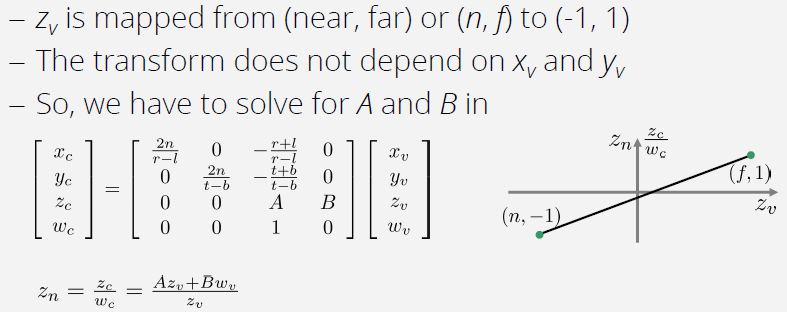
\includegraphics[scale=0.6]{image43.png}\\\\
Then, we can solve A and B and get the complete Projection Matrix
\begin{figure}
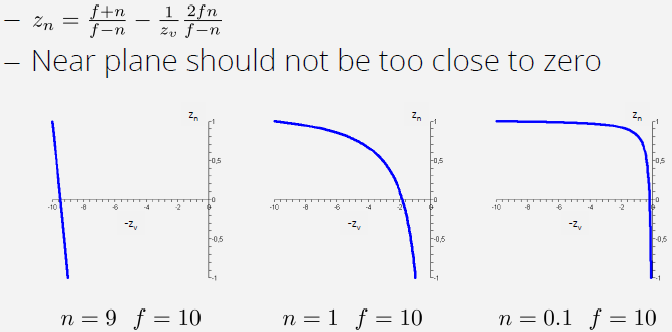
\includegraphics[scale=0.6]{image44.png}
\caption{Non-linear mapping of depth values}
\end{figure}

\subsubsection{Orthographic Projection}
\begin{figure}
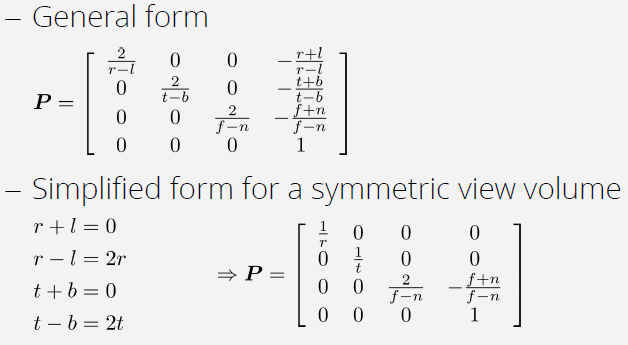
\includegraphics[scale=0.6]{image46.png}
\caption{Matrix general form}
\end{figure}

\subsection{Typical vertex transformations}
\begin{figure}[h!]
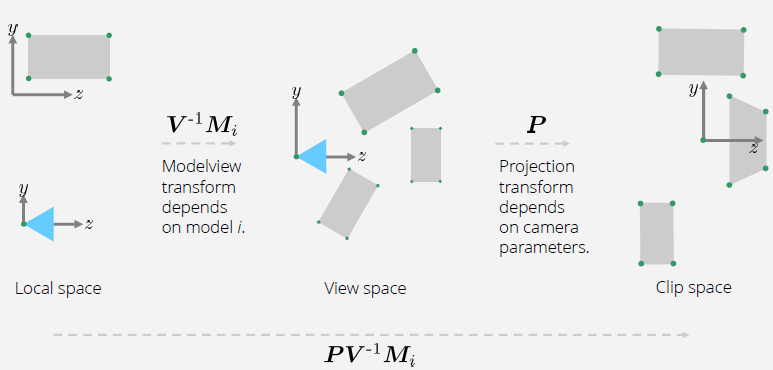
\includegraphics[scale=0.6]{image45.png}\\
\end{figure}
\begin{figure}[h!]
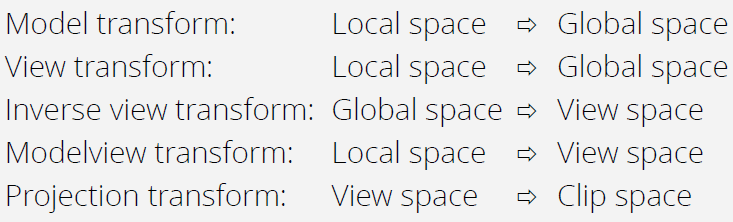
\includegraphics[scale=0.6]{image47.png}\\
\end{figure}

\begin{figure}[h!]
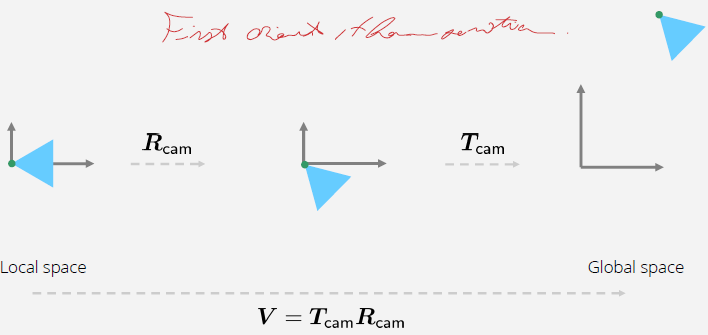
\includegraphics[scale=0.6]{image48.png}
\caption{Camera placement}
\end{figure}
\begin{figure}[h!]
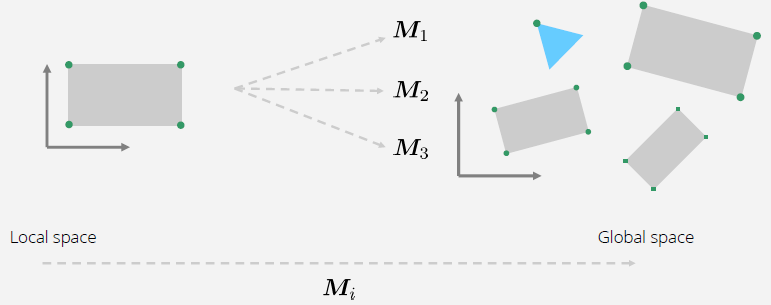
\includegraphics[scale=0.6]{image49.png}
\caption{Object Placement}
\end{figure}
\begin{figure}[h!]
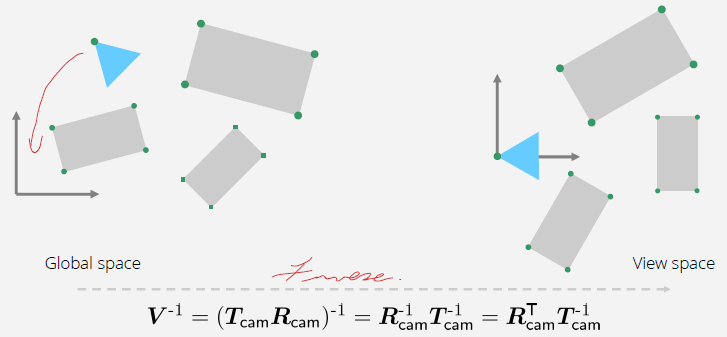
\includegraphics[scale=0.6]{image50.png}
\caption{View Transform}
\end{figure}
\begin{figure}[h!]
\includegraphics[scale=0.6]{image51.png}
\caption{Projection transform}
\end{figure}

\newpage
\section{Rasterization}
As we previously said, visibility can be resolved by ray casting or by rasterization. In particular, the second represent the computation of pixel positions in an image plane that represent a projected primitive. After that, we can solve visibility problem between various objects thanks to pixel positions.\\\\
\includegraphics[scale=0.6]{image52.png}\\\\
Rasterization is usually composed by three steps: \textbf{Rendering pipeline, Rasterization-based rendering, Rasterization.}\\

\subsection{Rasterization-based rendering}
\textbf{- Main stages:}\\
\subsubsection{1. Vertex processing.}
Scene modelling, placements.\\\\
\includegraphics[scale=0.6]{image54.png}\\\\
GPU rasterizers assume that all vertex positions are in clip / NDC space.\\
Only vertices inside the canonical view volume are processed, or the scene can be setup within the canonical view volume and rendered with parallel projection.\\
Position: Z component in NDC space is referred to as depth value, Color: Phong illumination model can be used, A parameer for rendering effects.\\\subsubsection{2. Rasterization.}
Fragments with attributes from primitives. In the Bresenham Line algorithm for Line rasterization, lines are represented as: F(x,y) = ax+by+c=0.\\\\
\includegraphics[scale=0.6]{image55.png}\\\\
\includegraphics[scale=0.6]{image56.png}\\\\
For what concern Polygons, compute intersections of non-horizontal edges with horizontal scanlines: y = y$\_$1 + 0.5. Fill pixel positions in between two intersections with fragments.\\\\
\includegraphics[scale=0.6]{image57.png}\\\\
\textbf{Attribute interpolation:} from vertices to fragments, anyway linear interpolation in view space cannot be realized by linear interpolation in clip space.\\\\
\includegraphics[scale=0.6]{image58.png}\\\\
w$\_$clip = Z$\_$view\\
\subsubsection{3. Fragment processing.}
Fragments attributes are processed and tested (making use of position, color, textures FB data etc.), then can be discarded or pass the test and used to update 
framebuffer attributes.\\\\
\begin{figure}[h!]
\includegraphics[scale=0.5]{image59.png}
\includegraphics[scale=0.5]{image60.png}
\caption{Example of texturing (e.g. Snake skin)}
\end{figure}
\textbf{- Tests:}\\
1. Scissor Test: check if fragment position is inside a specified rectangle.\\
2. Alpha Test: check range of the fragment alpha value. (e.g. for trasparency)\\
3. Stencil Test: check if FB stencil vlue fulfills a certain requirement.\\\\
\textbf{Example: Depth test}\\
Compare fragment depth value with the framebuffer depth value at the fragment position.\\\\
\includegraphics[scale=0.6]{image61.png}\\\\
\subsubsection{4. Fragment update}
Combine fragment color with framebuffer color (alpha value is used to set transparency level of images in order to make them mixing):\\\\
\includegraphics[scale=0.6]{image62.png}\\\\
\begin{figure}[h!]
\includegraphics[scale=0.6]{image53.png}\\\\
\caption{Complete overview.}
\end{figure}

\section{Parametric Curves}
In modelling, Parametric curves are used. Idea: specifying the curve with a small number of control points. It is computed as weighted sum of them ($p_i$).\\
\subsection{Polynomial curves}
\includegraphics[scale=0.6]{image63.png}
\subsection{Bézier Curves}
n+1 control points for degree n. First and last control point are interpolated, others are approximated.\\\\
\includegraphics[scale=0.6]{image64.png}
\includegraphics[scale=0.6]{image65.png}
\includegraphics[scale=0.6]{image66.png}\\\\
\textbf{- Property: }\\
1. Partition of unity: sum of t is 1.\\
2. Invariance under affine transformations:\\
\includegraphics[scale=0.5]{image68.png}
\includegraphics[scale=0.5]{image67.png}

\subsection{Bernstein Polynomials - Matrix Notation}
\includegraphics[scale=0.6]{image69.png}\\\\
\textbf{Polynomial bases:} canonical: {1,t,$t^2$,$t^3$}, elements must be linearly independent. \\\\
\includegraphics[scale=0.6]{image70.png}\\
\includegraphics[scale=0.6]{image71.png}\\\\
\textbf{General spline formulation: }piecewise polynomial function, x(t) = \textbf{GST}(t)
\subsubsection{Conversion from Canonical to Bézier}
\includegraphics[scale=0.6]{image72.png}\\\\
\subsection{Curve subdivision}
Given a curve from $p_0$ to $p_3$, generate two curves from $p_0$ to $x(t_{split})$ and from $x(t_{split})$ to $p_3$ given a value $0 \le t_{split} \le 1$.\\
\textbf{- Applications: } Rendering: \textit{subdivide a curve toward almost linear segments}, Modeling: \textit{modify a part of a curve.}\\
\includegraphics[scale=0.5]{image73.png}\\
\includegraphics[scale=0.5]{image74.png}\\
\includegraphics[scale=0.5]{image75.png}\\
\includegraphics[scale=0.5]{image76.png}\\\\

\section{Differential Curves}
\textbf{- Properties: }Derivatives, can be considered when connecting polynomials to splines.\\
\textbf{- Tangent: }Direction of a curve in that point.\\
\includegraphics[scale=0.5]{image77.png}\\\\
\textbf{- Velocity: }if t is interpreted as time, the derivative is the velocity.\\
\textbf{- Acceleration: }same but for the second derivative.\\
\includegraphics[scale=0.5]{image78.png}\\\\
\subsection{$C^k$ Continuity}
A parametric curve is $C^k$ Continuous if the first k derivatives exists and are continuous.\\
\includegraphics[scale=0.5]{image79.png}\\\\
\subsection{Piecewise polynomial curves}
Why to connect polynomial curves of lower degree to larger piecewise ones?\\\\
\includegraphics[scale=0.5]{image80.png}\\\\
\textbf{$G^k$ continuity: (Geometry continuity) }same velocity direction, proportional magnitude.\\\\
\subsubsection{Cubic Bézier Spline}
$C^0$ continuity: $p_3^{(i)}$ = $p_0^{(i+1)}$. Intermediate control points $p_1^{(i)}$, $p_2^{(i)}$ and $p_1^{(i+1)}$, $p_2^{(i+1)}$ can be used to obtain $C^1$ continuity.
\includegraphics[scale=0.5]{image81.png}\\\\
\subsubsection{Cubic Polynomial in Canonical Form}
\includegraphics[scale=0.5]{image82.png}
\includegraphics[scale=0.5]{image83.png}
\subsubsection{Cubic Hermite}
\includegraphics[scale=0.5]{image84.png}
\includegraphics[scale=0.5]{image85.png}\\
\includegraphics[scale=0.5]{image87.png}
\includegraphics[scale=0.5]{image86.png}\\\\
\subsubsection{Catmull-Rom Spline}
Variant of the Hermite Spline: formulate derivatives with control points.\\\\
\includegraphics[scale=0.5]{image88.png}
\includegraphics[scale=0.5]{image89.png}\\
\includegraphics[scale=0.5]{image90.png}\\\\
\section{Particle Fluids}
It is a topic about simulation.\\
\subsection{Particle simulation}
Estimate particles properties: $x_i^t$ and $v_i^t$
\subsection{Particle motion}
\includegraphics[scale=0.5]{91.png}\\\\
Computation of unknown future particle quantities from known current information.\\\\
\textbf{- Governing Equations for a particle: }\\
\textit{Newton's Second Law: }describe behavior of $x^t$ and $v^t$ in terms of their time derivative. \\
Given initial position and velocity, the problem is to estimate the next step (H can be seen as depending on frame rate. Smaller the step, smoother the animation.):\\
\begin{itemize}
\item \textbf{Explicit Euler Update: }\\
\includegraphics[scale=0.5]{image91.png}\\
\item \textbf{Verlet (Taylor approximations): }\\
\includegraphics[scale=0.5]{image92.png}
\end{itemize}
\subsection{Particle forces in a fluid}
\textbf{- Governing Equations for Fluid: }\\
Particle positions $x_i^t$ and the respective attributes are \textit{transported }with the local fluid velocity $v_i^t$, $\frac{dx_i^t}{dt}=v_ i^t$. Time rate of change of the velocity is governed by the Lagrange form of the Navier-Stokes equation (set of accelerations): \\
\includegraphics[scale=0.5]{image93.png}\\\\
\begin{itemize}
\item \textbf{-$\frac{1}{p_i^t}*gradient*p_i^t$}: Acceleration due to pressure differences, proportional to compression, particles are accelerated from areas with high pressure to lower pressure.
\item \textbf{$v*gradient^2*v_i^t$: }Acceleration due to friction forces between particles with different velocities.
\includegraphics[scale=0.5]{image94.png}
\end{itemize}
\subsection{Smoothed Particle Hydrodynamics SPH}
Interpolates quantities at arbitrary positions and approximates the spatial derivatives with a finite number of samples.\\\\
\includegraphics[scale=0.5]{image95.png}\\\\
Quantity $A_i$ is approximated with a set of known quantities $A_j$ at sample positions $x_j$:
\includegraphics[scale=0.5]{image96.png}\\
$W_{ij}$ is a kernel function that weights the contributions of sample positions $x_j$ according to their distance to $x_i$.\\
\includegraphics[scale=0.5]{image97.png}\\
\subsection{SPH for particle fluids}
\subsubsection{Density}
Explicit SPH form (Useful for force computation):\\
\includegraphics[scale=0.5]{image98.png}\\\\
\subsubsection{Pressure}
Quantifies fluid compression:\\
$p_i = max(k(\frac{\rho_i}{\rho_0} -1),0)$ if the frac is $>1$ then there is compression. Pressure acceleration with SPH.\\
\includegraphics[scale=0.5]{image99.png}\\\\
\begin{figure}
\includegraphics[scale=0.5]{image100.png}
\caption{Discretizations}
\includegraphics[scale=0.5]{1.png}
\caption{SPH Fluid Solver}
\end{figure}
\subsection{Neighbor search}
Particles are stored in cells, cell size equals the kernel support of a particle. Compute unique cell identifier per particle, sort particles with respect to cell identifier, map cells to a hash table.\\\\
\includegraphics[scale=0.5]{1.png}\\\\

\subsection{Boundary handling}
Boundaries are sampled with particles that contribute to density, pressure and pressure acceleration.\\\\
\includegraphics[scale=0.5]{3.png}\\
\includegraphics[scale=0.5]{4.png}\\\\
\textbf{- Pressure at Boundary Samples: }\\
\includegraphics[scale=0.5]{5.png}\\
\textbf{- Mirroring (\textit{$p_{ib}=p_i$}): }\\
\includegraphics[scale=0.5]{6.png}\\
\subsection{Visualization}
\subsubsection{ISO-surface reconstruction}
\includegraphics[scale=0.5]{7.png}\\
\textbf{Initialization: } Density computation using SPH.\\
\includegraphics[scale=0.6]{8.png}
\includegraphics[scale=0.6]{9.png}
\includegraphics[scale=0.6]{10.png}\\
\textbf{Classification: } $\rho_i \le 0.5 \rho^0=>$ \textbf{out}, otherwise \textbf{in}.
\newpage


\part{Image Processing}
\newpage

\section{Introduction and Image basics}

\textbf{Digital images: }matrix of pixels, defined by an intensity values ($I_{ij}: (\Omega \subset R^2)-> R$).\\

Matching human visual capabilities means to solve a large part of the AI/ML problem.\\
Image content is defined by the spatial arrangement of intensities. It is not sufficient to treat images as vectors and to analyze these vectors.\\
\includegraphics[scale=0.7]{11.png}\\\\
\textbf{How it works in our brain: }The retina significantly reduces the amount of data before it is sent to the brain. In the visual cortex the data is then expanded again. In lower cortical areas (especially V1), neurons respond only to signals in a very small local area (receptive field). In higher cortical areas, the receptive fields get larger and larger due to integration of information from lower areas. \\

\subsection{Imaging model}
\begin{itemize}
\item \textbf{Pinhole camera}
Objects points (X,Y,Z) are projected to image points (x,y) by $x=f \frac{X}{Z}$, $y=f \frac{Y}{Z}$\\
\includegraphics[scale=0.7]{12.png}
\item \textbf{Optical camera}
Large aperture and sharpness possible at a certain depth. Thin lenses: $\frac{1}{S_1}+\frac{1}{S_2}=\frac{1}{f}$\\
\textbf{Wide lenses:} focal length depends on orientation and color.
\end{itemize}

\subsection{Image representation}
\begin{itemize}
\item \textbf{gray value images}\\
Image is a continuous function: I: ($\Omega \subset R^2$) $->$ R. $\Omega$ is the image domain (usually rectangular).\\
\includegraphics[scale=0.7]{13.png}
\item \textbf{Sampling}
Intensities are only given on a pixel grid. Grid points are called pixels. If true spacing not known, then grid size of input image set to \textit{h=1}.\\
The number of grid points to represent the discrete image is called the\textbf{ image resolution}. Reducing the number of grid points is called \textbf{downsampling}. Increasing the number of grid points is called \textbf{upsampling}.\\
A discrete signal can only represent frequencies up to a certain limit Nyquist frequency, ignorance of the Nyquist frequency leads to aliasing artifacts (e.g.: straight lines become stepped). 
\textbf{- Nyquist-Shannon theorem}\\
\begin{quote}
An input signal can be reconstructed from samples in a unique way if the
sampling rate is at least two times the bandwidth of the input signal.
\end{quote}

\item \textbf{Downsampling}
\textbf{Decanting operator:} ensures minimum smoothing necessary to avoid aliasing. In case of overlap, intensity distribution to both cells according to the overlap ratio. 
\item \textbf{Upsampling} 
\textbf{Bilinear interpolation: }weighted average of neighboring pixels. Project fine grid point to available coarse grid. Compute weighted average along x-axis: $a_j=(1-\alpha)I_{i,j}+\alpha I_{i+1,j}$\\
Same for y-axis with $\beta$. Can be extended to arbitrary dimensions (trilinear interpolation). 
\end{itemize}

\subsection{Quantization}
To represent a digital image we have to discretize the co-domain: $R->{1,...,N}$, usual image formats have 256 grey scales (8 bpp).\\
\includegraphics[scale=0.7]{14.png}
\subsection{Types of images}
\textbf{Standard” images:} image domain is two-dimensional, co-domain one-dimensional (gray scale).\\
\textbf{Matrix-valued images: }Diffusion tensor MRI: flow preferences of water molecules, Each voxel (volume element) comprises a 3x3 matrix.\\

\section{Noise, basic operations and filters}
Noise is a disturbance of the image data. With actual tools noise anymore exists. Rather than removing noise, make sure the model can deal with noise.\\
\textbf{- Types of noise: }\\
\begin{itemize}
    \item \textbf{Additive noise: }\\
    gray values and noise are independent: $I_{ij} = I_{ij}+n_{ij}$\\
    \includegraphics[scale=0.4]{15.png}
    \item \textbf{Gaussian noise: }\\
    Density function: $G_\sigma(x)=\frac{1}{\sqrt{2\pi \sigma^2}}exp(-\frac{(x-\mu)^2}{2\sigma^2})$\\
    Good approximation in many practical situations, In particular: thermic sensor noise in CCD cameras.\\
    \includegraphics[scale=0.4]{16.png}
    \item \textbf{Multiplicative noise:}\\
    Signal dependent: $I_{ij}=I_{ij}^*(1+n_{ij})$\\
    More difficult to handle, better transforming the image with log, noise becomes additive noise, apply backtransform to denoised image: $I_{ij}^*=exp \log I_{ij}^*$
    \item \textbf{Impulse noise}\\
    A certain percentage of pixels is replaced by fixed values, caused, for instance, by pixel defects of CCD chips.
    \item \textbf{Uniform noise}\\
    A certain percentage of pixels is replaced by uniformly distributed random variables. Very unpleasant noise, no a-priori knowledge in the noise model.
\end{itemize}
\textbf{- Signal to Noise Ratio (SNR)}\\
Quantitative measure for the degradation of an image $I$ versus a noise-free version $I^*$\textbf{ (ground truth)}. Based on the variance of the image versus the variance of the noise.\\
\includegraphics[scale=0.3]{17.png}\\\\
For small ranges, peak is better.
\textbf{- Point operations}\\
The most straightforward way to enhance an image is to treat each pixel
independently: $u_{ij} = f(I_{ij})$, Example: changing brightness:\\
$u(x,y)=I(x,y)+b$, darkening for b<0.\\\\
\textbf{- Contrast enhancement: }\\
$u(x,y)=aI(x,y)$\\
$a>1$, contrast attenuation for $a<1$, clip values greater than the allowed range.\\\\
\textbf{- Gamma correction: }\\
Cameras have different response curves that human eye: $I \propto $ (is proportional) $ I^\gamma$.\\
Compensation: $f(I(x,y)) = I_{max}(\frac{I(x,y)}{I_{max}})^\gamma$\\
Dark areas become brighter without leading to oversaturation in the brighter areas.\\
With $\gamma$ greater than 1, the image get darker, and viceversa.\\\\
The \textbf{gray value histogram} contains the number of pixels in the image that
have a certain gray value. The equalization is done to have all grey values equally frequent.\\\\
\textbf{- Difference image:}\\
Subtract greyvalues of two subsequent images $\longrightarrow I_\Delta = |I_1-I_2|$. (Can be used for detecting parts of moving objects in static scenes).\\
\textbf{- Background substraction:} \\
Take an image of a background, the difference image indicates the object. It can be used for object tracking and segmentation of a person in front of a static background.\\
$I_\Delta = \frac{1}{3}\sum_{k=1}^3|I_{k,1}-I_{k,2}|$\\\\
\textbf{Linear filters, convolution theorem}\\
Filters take neighboring pixels into account to improve the signal. Since filters are designed in the Fourier domain we will use \textbf{convolution theorem: }$F(f)F(h)=F(f*h)$, with F - Fourier transform. In image processing, filters are diectly designed in Spatial domain because: it is easier to handle and to generalize to nonlinear filters.\\
x' is the shift, convention of the filter to use -x'.
\begin{itemize}
    \item \textbf{Linear:} $(f*h)(x) = \int h(-x')f(x+x')dx'$
    \item \textbf{2D:} $(I*h)(x,y) = \int h(-x',-y')I(x+x',y+y')dx'dy'$
\end{itemize}
\textbf{- Properties: }
\begin{itemize}
    \item \textbf{Linearity: } $(\alpha f+\beta g)*h=\alpha (f*h)+ \beta (g*h)$
    \item \textbf{Shift invariance: }$f(x)*g(x+\delta) = (f*g)(x+\delta)$
    \item \textbf{Commutativity: }$f*g = g*f$
    \item \textbf{Associativity: }$(f*g)*h = f*(g*h)$
    \item \textbf{Correlation: }$f(x)\star h(x) = \int h(x')f(x+x')dx'$
\end{itemize}
\includegraphics[scale=0.35]{19.png}\\\\
Separable filters can be implemented via successive 1D convolutions (associativity of convolution). This reduces the computational complexity of the convolution from $O(NMnm)$ to $O(NM(n+m))$.\\
\subsection{Gaussian filtering}
Used for image smoothing, the convolution filter is implemented with a Gaussian kernel of width $\sigma$: $G_\sigma(x)=\frac{1}{\sqrt{2\pi\sigma}}exp(-\frac{x^2}{2\sigma^2})$, the Gaussian filter is separable, the smoothed image can be derived as $I^{\sim}(x,y)=I(x,y)*G_\sigma(x,\dot)*G_\sigma(\dot,y)$\\
\textbf{Complexity: }$O(NM\sigma)$, in Fourier domain: $O(NM\log(NM))$\\\\
\includegraphics[scale=0.2]{20.png}
\includegraphics[scale=0.2]{21.png}\\\\
The image domain $\Omega$ is generally not an infinite domain but has boundaries $\delta\Omega$.\\
\textbf{Boundary types: }
\begin{itemize}
    \item \textbf{Dirichlet boundary conditions:} I(x,y)=0
    \item \textbf{Homogeneous Neumann boundary conditions:} $\frac{\delta}{\delta n} I(x,y)=0$, where n is the outer normal vector on $\delta\Omega$ and $\frac{\delta I}{\delta n}= n^T\nabla I$ is the directional derivative. 
\end{itemize}
Neumann are preferred because they have nicer properties. They are obtained by mirroring the image at the boundary.\\
\subsubsection{Why to prefer Gaussian to box filter?}
\begin{itemize}
    \item \textbf{a)} The box filter is not separable
    \item \textbf{b)} The Gaussian filter is rotationally invariant, the box filter is not
    \item \textbf{c)} Of course we prefer a box filter
\end{itemize}
\subsection{Box filter}
\includegraphics[scale=0.35]{22.png}\\\\
Simple averaging of neighbouring values, \textbf{but} results are not smooth and not rotationally invariant. The advantage is that convolution with a large kernel is much more efficient, since\\
\includegraphics[scale=0.35]{23.png}\\
Complexity O(NM) independent of $\sigma$\\\\
\includegraphics[scale=0.2]{24.png}
\includegraphics[scale=0.2]{25.png}\\\\
Anyway, box filters have some relations to Gaussian filter, since iterating the convolutions of the box kernel with itself make the filter similar to gaussian.\\
\textbf{- Central limit theorem in statistics: }iterated averaging kernels (= positive kernels) converge to Gaussians.\\
\subsection{Recursive filter}
Recursively propagate information in both directions of the signal:\\
\includegraphics[scale=0.35]{26.png}\\
Recursive filter approximates Gaussian convolution, filter is separable and rotationally
invariant. \textbf{Relation:} $\alpha \sigma = \frac{5}{2\sqrt{\pi}}$.\\
Complexity O(NM) is independent of $\alpha$\\\\
\includegraphics[scale=0.35]{27.png}\\
An important aspect of image processing is the local change of intensities. In continuous functions it is given by the derivative. In multidimensional is the gradient.\\
Differentiability of images is ensured by combining the derivative with a small amount of Gaussian smoothing $->$ Gaussian derivatives.\\
The derivative can be applied to the image or to the Gaussian. Gaussian funcions is $C^\infty$, so infinitly differentiable. A common mask for the first derivative is (-1/2, 0, 1/2) (\textbf{Central difference}).\\
Instead for higher order derivatives, use \textbf{Laplace filter}, based on second derivatives.\\
\includegraphics[scale=0.35]{28.png}\\\\
Another way to detect edges is by the gradient magnitude (based on first derivatives): $|\nabla I|=\sqrt{I^2_x+I^2_y}$.\\\\
\includegraphics[scale=0.3]{29.png}\\\\


\section{Energy minimization}
\textbf{- Concept: }\\
\textbf{1.} Formalize your model as an optimization problem: $E(x)=A_1(x)+,...,+A_n(x)$\\
\textbf{2.} Solve the optimization problem: $x^*=argmin_xE(x)$\\
E(x) is called energy (in ML loss funciton).\\
\textbf{- Example: image denoising} \\\\
\includegraphics[scale=0.3]{30.png}\\\\
\textbf{- Advantages: }transparency, optimality, compatibility.\\
Global optimization is often hard. Heuristics can obliterate the initial transparency of the model.\\
\begin{equation}
E(u_{i,j})=\sum_{i,j}((u_{i,j}-I_{i,j})^2+\alpha((u_{i+1,j}-u_{i,j})^2+(u_{i,j+1}-u_{i,j})^2))
\end{equation}
To minimize the function: derivatives must be zero:
\begin{equation}
\frac{\delta E}{\delta u_{i,j}}=2(u_{i,j}-I_{i,j})+2\alpha(u_{i,j}-u_{i-1,j})-2\alpha (u_{i+1,j}-u_{i,j})+2\alpha(u_{i,j}-u_{i,j-1})-2\alpha(u_{i,j+1}-u_{i,j})=0
\end{equation}
Necessary conditions:\\
\begin{equation}
\frac{\delta E}{\delta u_{i,j}}=(u_{i,j}-I_{i,j})+\alpha(u_{i,j}-u_{i-1,j})-\alpha (u_{i+1,j}-u_{i,j})+\alpha(u_{i,j}-u_{i,j-1})-\alpha(u_{i,j+1}-u_{i,j})=0
\end{equation}
Can be written as:\\
\includegraphics[scale=0.3]{31.png}\\\\
Since A is Positive definite $\rightarrow$ the inverse $A^{-1}$  exists and we can solve for u.\\
\subsection{Convexity}
\textbf{- Convex functions:} Positive curvature, global minimum is unique.\\
\textbf{- Non-convex functions:} Many local minima, global minimum not unique.\\
\includegraphics[scale=0.3]{32.png}\\\\
\textit{\textbf{Theorem:}} every convex combination of (strictly) convex functions is again (strictly) convex.\\
To solve the linear system, an iterative solver is needed\\\\
\includegraphics[scale=0.3]{33.png}
\subsection{Jacobi Method}
Decompose A = D+M (D: diagonal part, M: off-diagonal part)\\
$Ax=b \leftrightarrow (D+M)x=b \leftrightarrow Dx=b-Mx$\\
$D^{-1}$ can be computed very easily: just replace the diagonal elements by their inverse.\\
Now compute x iteratively starting by $x^0$ and: $x^{k+1}=D^{-1}(b-Mx^k)$, until the residual $r^k=Ax^k-b$ is under a threshold. When is 0 $\rightarrow$ converged.\\
\textbf{- Advantages: } simple and parallelizable, \textbf{- Disadvantages: } slow, convergence only at $\infty$, computation not in place.
\subsection{Gauss-Seidel Method}
Split M into lower triangle and upper:\\
$Ax=b \leftrightarrow Dx=b-Lx-Ux$\\
During iteration, use new values with the lower triangle:\\
$x^{k+1}=D^{-1}(b-Lx^{k+1}-Ux^k)$\\
In-place computation, recursive propagation of information is faster\\
\subsection{Successive over-relaxation (SOR)}
Emphasize the Gauss-Seidel idea by over-relaxing the new solution
$x^{k+1}=(1-\omega)x^k+\omega D^{-1}(b-Lx^{k+1}-Ux^k)$\\
Converges for positive or negative definite matrices, if $\omega \in (0,2)$. Over relaxation for $\omega >1$, under for $\omega <1$.
\subsection{Conjugate gradient (CG)}
Two vectors are conjugate if they are orthogonal with respect to A: $<u,v>_A=u^TAv=0$.\\
\includegraphics[scale=0.3]{34.png}\\
Start with some initial point $x^0$, Let $p_0$ be the residual $r_0=b-Ax^0$. This is the gradient of: $E(x)=\frac{1}{2}x^TAx-b^Tx$ the minimizer of which is $x^*$\\
Then, iteratively compute:\\
\includegraphics[scale=0.3]{35.png}\\
Stop when residual is small.\\
A must be symmetric and definite, usually we don't consider exact solution. Sometimes, preconditioners $P^{-1}$ are used to have small condition number for $P^{-1}A$\\
$Ax = b \leftrightarrow P^{-1}Ax=P^{-1}b$
\subsection{Multigrid methods}
All previous linear solvers have the drawback that they only act locally due to the sparsity of the matrix. \textbf{Idea: }regar the system from a coarser point of view. Faster.
\subsubsection{Unidirectional (cascadic)}
\textbf{1.} Create downsampled versions of the linear system\\
\textbf{2.} Compute first approximate solution at the coarse grid (e.g. with SOR)\\
\textbf{3.} Take upsampled result as initial guess for the next finer grid\\
\textbf{4.} Refine result there (again with SOR)\\
\textbf{Advantages: }Fast and simple, \textbf{Disadvntages: }Coarse level doesn't approximate so well.
\subsubsection{Correcting (bidirectional)}
\textbf{1.} Do not downsample the image but the error\\
\textbf{2.} Compute first solution at fine grid\\
\textbf{3.} Correct error at coarse grid\\
\textbf{4.} Refine result at finer grid\\\\
\includegraphics[scale=0.3]{36.png}\\
\subsubsection{Full multigrid}
\textbf{1.} Combination of cascadic and correcting multigrid\\
\textbf{2.} Start at coarse grid with downsampled image\\
\textbf{3.} At each finer level apply a W-cycle\\\\
\includegraphics[scale=0.3]{37.png}\\

\section{Variational Methods}
\subsection{Discrete/Continuous energies}
Continuous formulation: $u^*(x)=argmin_{u(x)}E(u(x))$, with $u(x):\Omega \rightarrow R$.\\
The energy function becomes an energy functional, optimization is based on the calculus of variation. \\
\textbf{- Advantage of continuous energies:}\\
It is not ensured that discrete energy is consistent with the continuous one. \\
\textbf{- Disafvantages: } Gradients have to be computed.
\subsection{Consistency}
Discretizatization of continuous can lead to errors. \\
\begin{quote}
A discretization is called consistent if it converges to the continuous model with finer grid sizes.
\end{quote}
\includegraphics[scale=0.3]{38.png}\\
In continuous field, to calculate variation, we need Gâteaux derivative.\\
A functional maps each element u of a vector space to a scalar E(u).\\
The Gâteaux derivative generalizes the directional derivative to infinite-dimensional vector spaces.\\
\includegraphics[scale=0.3]{39.png}\\\\
Back to our Denoising example, in the continuous field, it would be:\\
\includegraphics[scale=0.3]{40.png}\\
The optimization problem is on the funciton, necessary condition for a minimum:\\
$\frac{\delta E(u)}{\delta u}_h = 0$\\
\includegraphics[scale=0.3]{41.png}\\
\includegraphics[scale=0.3]{42.png}\\
These boundary conditions are called natural boundary conditions as they naturally emanate from the Gâteaux derivative. In the special case here, they coincide with Neumann boundary conditions.\\
\includegraphics[scale=0.3]{43.png}\\
Same linear solvers can be applied. The two different discretization stages do not always lead to the same algorithm.\\\\
\includegraphics[scale=0.3]{44.png}
\includegraphics[scale=0.3]{45.png}\\\\
A quadratic regularizer leads to blurred edges, so we must do some exceptions (outliers) with non-quadratic regularizers. \\
\textbf{- Statistical interpretation}\\
Energy minimization can also emerge from a probabilistic approach taking into account likelihoods and prior probablities: $p(u|I)=\frac{p(I|u)p(u)}{p(I)}$, find u that maximizes (MAP), marginal p(u can be ignored when maximizing).\\
How is it useful? Turn maximization of the probability into minimization of the negative logarithm $\rightarrow$ energy minimization problem\\
\includegraphics[scale=0.3]{46.png}\\\\
Other noise models lead to different penalizers in the energy functional, excepting outliers we can replace Gaussian by Laplace.\\
\includegraphics[scale=0.3]{47.png}\\\\
\includegraphics[scale=0.3]{48.png}\\\\
The Euler-Lagrange equation is nonlinear in the unknowns, discretization leads to a nonlinear system of equations. A general way to minimize discrete or continuous energies is by gradient descent.\\
\textbf{Iterative method:} start with an initial value, iteratively move in direction of
largest decrease in energy (negative gradient direction).\\\\
\includegraphics[scale=0.3]{49.png}
\includegraphics[scale=0.3]{50.png}\\\\
\textbf{- Gradient descent: }\\
\includegraphics[scale=0.3]{51.png}\\
\includegraphics[scale=0.3]{52.png}\\
This is the \textbf{lagged diffusivity} and has been proven to converge if the linear system in each step is solved exactly. Increased efficiency, Much faster than gradient descent.\\\\
\includegraphics[scale=0.3]{53.png}
\newpage
\section{Motion Estimation}
The problem here is to estimate the position of the pixels of an image moving. We seek a vector field (u,v)(x,y,t) \textbf{Optical flow field} that describe the motion at t. It can be used for detection or segmentation of objects by comparing the object motion and the background motion $\rightarrow$ motion segmentation (separate objects from the background), or for 3D motion of objects (\textbf{scene flow}). Optical flow can also help estimate the 3D structure of objects. This is called \textbf{structure from motion.}\\\\
\includegraphics[scale=0.3]{54.png}\\\\
What is perceived, can be different from the reality. The neighborhood (aperture) determines the solution of the optical flow. Therefore, the ambiguity is also called the aperture problem.\\
\textbf{Assumption:} gray value of a moving pixel is constant: $I(x+u,y+v,t+1)-I(x,y,t)=0$.\\
To ease optical flow estimation, we can linearize the first expression with a Taylor expansion:
\begin{center}
$I(x+u,y+v,t+1)=I(x,y,t)+I_xu+I_yv+I_t+O(u^2,v^2)$, $I_x$ x-derivative of the image.
\end{center}
This leads to the (linearized) optic flow constraint:
\begin{center}
$I_xu+I_yv+I_t=0$
\end{center}
\subsection{Lucas-Kanade Method}
Regarding a single pixel, we cannot uniquely determine its flow vector. There is only one equation, but two unknowns.  The Lucas-Kanade method assumes that the motion is constant within a local neighborhood. We then obtain multiple equations for the two unknowns:
\begin{equation}
I_x(x',y',t)u+I_y(x',y',t)v+I_t(x',y',t)=0$, $\forall x',y'\in R(x,y)
\end{equation}
It has not a solution anymore, so we just try to minimize the total square error:\\
\begin{center}
$argmin_{u,v} \sum_{x,y\in R}(I_x(x,y)u+I_y(x,y)v+I_t(x,y))^2$
\end{center}
\includegraphics[scale=0.3]{55.png}\\
We can also use a Gaussian Window (the bigger the window, the less the reliability). It leads to a convolution:\\
\includegraphics[scale=0.3]{56.png}\\
A unique solution will be obtained only if the system is \textit{not singular}(2 non-zero eigenvalues).\\
\textbf{- Drawbacks of the Lucas-Kanade method:} locally constant motion is not realistic, There are no direct constraints on the smoothness of the resulting flow field.\\
\textbf{- Advantages:} fast and simple.\\
\includegraphics[scale=0.3]{57.png}\\\\
In contrast with Lucas-Kanade, global methods have a global dependency between points due to a global smoothness assumption.
\subsection{Horn-Schunck model}
A global solution is usually derived with variational methods.
Same assumption: gray value constancy leading to the optic flow constraint. \\
\begin{equation}
I_xu+I_yv+I_z=0
\end{equation}
The second assumption is different. The Horn-Schunck model assumes global smoothness of the flow field:
\begin{equation}
|\nabla u|^2+|\nabla v|^2 \rightarrow min
\end{equation}
Both construct the energy functional:
\begin{equation}
E(u,v)=\int_{\Omega}(I_xu+I_yv+I_z)^2+\alpha(|\nabla u|^2+|\nabla v|^2) dxdy
\end{equation}
That's quadratic so the function is convex (unique optimum). To find the minimizer use calculus of variation.\\
\includegraphics[scale=0.3]{58.png}\\\\
\includegraphics[scale=0.3]{59.png}\\\\
This system can be written in matrix-vector notation: $A^hw=b$, where $w=()u,v$. As in the denoising case, the system matrix is sparse with only few diagonals different from zero.\\
\includegraphics[scale=0.3]{60.png}\\
The data term contributes only to block main diagonals. The smoothness term has four additional block off-diagonals.\\\\
\includegraphics[scale=0.3]{61.png}\\\\
An established measure of how accurately the optical flow has been estimated is the \textbf{average angular error}. \\
The average angular error measures the 3D angle between the correct and the estimated flow vectors:
\begin{equation}
AAE = \frac{1}{n} \sum_{i=1}^n arccos(\frac{(u_c)_i u_i+(v_c)_i v_i+1}{\sqrt{((u_c)_i^2+(v_c)_i^2+1)(u_i^2+v_i^2+1)}})
\end{equation}
An alternative is the end point error: EPE = $\frac{1}{n}\sum_{i=1}^n\sqrt{(u_i-(u_c)_i)^2+(v_i-(v_c)_i)^2}$\\\\
\textbf{- Limitation of Horn-Schunck model}\\
\includegraphics[scale=0.3]{62.png}
\newpage
\section{}


























\end{document}
